\section{Experimentación}

\subsection{Descripción de la Experimentación}

\clearpage

\subsection{Resultados de la Experimentación}

\subsubsection{Fichero brain\_gse15824.csv}

\begin{table}[htp]
    \small
    \centering
    \begin{tabularx}{\columnwidth}{Y Y}
        ACC       & AUAC    \\\hline
        $0.757$   & $0.764$ \\\hline
    \end{tabularx}
    \caption{Resultados globales para el fichero brain\_gse15824.csv.}
    \label{tab:4}
\end{table}

\begin{table}[htp]
    \small
    \centering
    \begin{tabularx}{\columnwidth}{l c c c c}
                &  Astrocytoma  & Glioblastoma & Oligodendrioglioma   & Glioblastoma-cell-line   \\\hline
        TPR     &  $0.500$      & $1.000$      & $0.286$              & $1.000$                  \\\hline
        TNR     &  $0.966$      & $0.720$      & $0.967$              & $1.000$                  \\\hline
        PPV     &  $0.800$      & $0.632$      & $0.667$              & $1.000$                  \\\hline
        NPV     &  $0.875$      & $1.000$      & $0.853$              & $1.000$                  \\\hline
        LR+     &  $14.500$     & $3.571$      & $8.571$              & -                        \\\hline
        LR-     &  $0.518$      & -            & $0.739$              & -                        \\\hline
        DOR     &  $28.000$     & -            & $11.600$             & -                        \\\hline
        YI      &  $0.466$      & $0.720$      & $0.252$              & $1.000$                  \\\hline
        MCC     &  $0.561$      & $0.674$      & $0.362$              & $1.000$                  \\\hline
        DP      &  $0.798$      & -            & $0.587$              & -                        \\\hline
        $F_{1}$ &  $0.615$      & $0.774$      & $0.400$              & $1.000$                  \\\hline
        MK      &  $0.675$      & $0.632$      & $0.520$              & $1.000$                  \\\hline
        BCR     &  $0.733$      & $0.860$      & $0.626$              & $1.000$                  \\\hline
        GM      &  $0.695$      & $0.849$      & $0.526$              & $1.000$                  \\\hline
        OP      &  $0.547$      & $0.648$      & $0.294$              & $1.000$                  \\\hline
        Jaccard &  $0.444$      & $0.632$      & $0.250$              & $1.000$                  \\\hline

    \end{tabularx}
    \caption{Resultados agrupados por clase para el fichero brain\_gse15824.csv.}
    \label{tab:6}
\end{table}

\clearpage

\begin{figure}[htp]
    \centering
     \subfloat[Curva ROC]{
       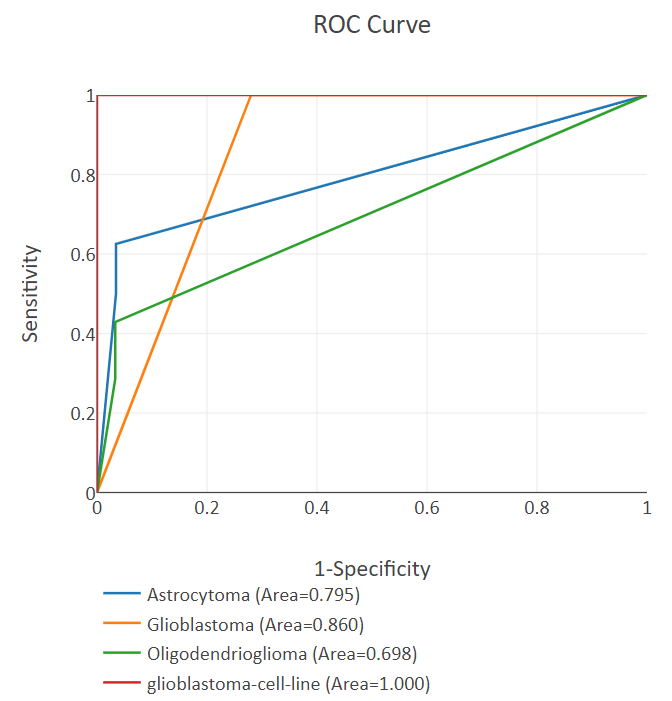
\includegraphics[width=0.4\textwidth]{brain_gse15824_ROC.PNG}}
     \subfloat[Curva A]{
       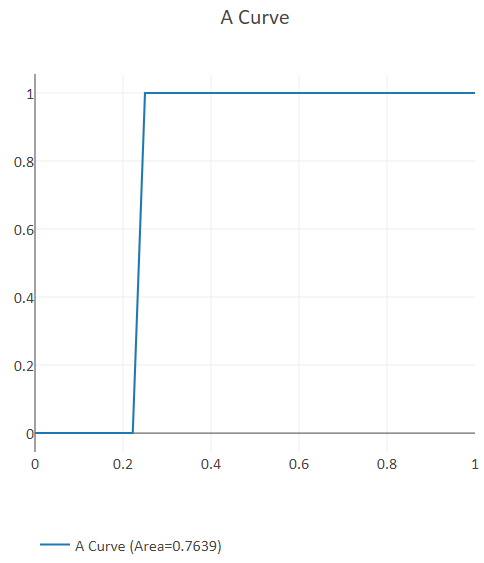
\includegraphics[width=0.4\textwidth]{brain_gse15824_A_CURVE.PNG}}
    \caption{Curvas obtenidas para el fichero brain\_gse15824.csv.}
    \label{fig:3}
\end{figure}

\bigbreak

\lipsum[1]

\clearpage

\subsubsection{breast\_gse45827.csv}

\begin{table}[htp]
    \small
    \centering
    \begin{tabularx}{\columnwidth}{Y Y}
        ACC       & AUAC    \\\hline
        $0.757$   & $0.764$ \\\hline
    \end{tabularx}
    \caption{Resultados globales para el fichero breast\_gse45827.csv.}
    \label{tab:7}
\end{table}

\begin{table}[htp]
    \small
    \centering
    \begin{tabularx}{\columnwidth}{X X X X X X X}
                &  Her  & Basal & Cell\_line & Luminal\_a & Luminal\_b & Normal    \\\hline
        TPR     &       & $0.1$ &           &           &           &           \\\hline
    \end{tabularx}
    \caption{Resultados agrupados por clase para el fichero breast\_gse45827.csv.}
    \label{tab:8}
\end{table}

\clearpage